\documentclass[dvipdfmx,a4paper]{jreport} % dvipdfmxオプションを追加
\usepackage{amsmath,amssymb}
\usepackage{graphicx}
\usepackage{url} % ウェブサイトのURLをきれいに表示するため
\usepackage{multicol} % 必要であれば多段組用
\usepackage{caption} % 図表のキャプション設定
\usepackage{subcaption} % subfigure環境用
\usepackage{float} % [H]オプションを使うため

% 日本語設定
\usepackage[utf8]{inputenc}
\usepackage[T1]{fontenc}
\usepackage{otf}
\usepackage[ipaex]{pxchfon} % IPAexフォントを使用 (pxgothicの代わりに推奨)
\usepackage{url}
\usepackage{booktabs}
\usepackage{geometry}
\geometry{a4paper,
    top=30mm,
    bottom=30mm,
    left=25mm,
    right=25mm
}

% タイトルページの作成
\makeatletter
\def\titlepage{%
\thispagestyle{empty}%
\begin{center}%
    \vspace*{\fill}%
    {\huge \bfseries 2D水槽における波浪中動揺試験 \\}%
    \vspace{2cm}%
    {\large 実施日時:7月15日\\}%
    \vspace{1cm}%
    {\large 2班\\}%
    \vspace{1cm}%
    {\large 学籍番号:08C23031\\}%
    \vspace{1cm}%
    {\large 氏名:古賀 光一朗 \\}%
    \vspace*{1cm}%
    {\large 共同実験者:藏藤 大貴, 桑原 陽, 小柳 拓未, 酒井 陸杜, 佐藤 創大, 竹内 里玖, 武原 翔生, 田中 健太郎, 杉山 寛樹}
    \vspace{\fill}
\end{center}%
}
\makeatother

\begin{document}

\titlepage

---

\chapter{試験の目的}
この試験の目的は、波浪中における船や海洋構造物といった\textbf{浮体の運動特性を理解すること}である。浮体は波の周期によって様々な揺れ方をするので時には転覆する危険もあり、安全な設計のためには、波の中で浮体がどう動くかを知っておく必要がある。\\
具体的には、二次元水槽で浮体模型を使って\textbf{波浪中動揺試験}を行う。この試験で目指すのは、以下の点である。
\begin{itemize}
    \item 流体力と浮体の運動の関係を理解する
    \item 波と浮体の運動の関係を理解する
    \item 水槽試験の基礎技術を習得する
    \item 試験結果を科学的なレポートにまとめる
\end{itemize}

\chapter{理論}
\section{運動振幅比 $|X|/\zeta_a$ の導出}

まず、浮体の揺れの大きさを表す $|X|$ と、やってくる波の振幅を表す $\zeta_a$ の比、つまり $|X|/\zeta_a$ をどうやって求めるか考える

\subsection{前提}
    簡単のために、波の振幅は小さく、やってくる波は規則波と仮定する。\\この波の揺れは、(\ref{eq:zeta01})式のようにコサイン関数で表せる。
    \begin{equation}
    \label{eq:zeta01}
        \zeta (t) = \zeta_a \cos \omega t = \text{Re}[\zeta_a e^{i\omega t}]
    \end{equation}
    \begin{itemize}
        \item $\zeta_a$ :波の片振幅(波の高さの半分)
        \item $\omega$ :その波の振動の速さ(円周波数)
    \end{itemize}

\subsection{運動方程式を立てる}
    物体の運動と言えば、基本はニュートンの第二法則である。つまり「質量 × 加速度 = 力」。これを浮体に当てはめると、式(\ref{eq:dynamics})になる。
    \begin{equation}
    \label{eq:dynamics}
        m\ddot{x}(t) = f(\ddot{x}, \dot{x}, x, t)
    \end{equation}
    \begin{itemize}
        \item $m$:浮体の質量
        \item $x(t)$:浮体の上下の揺れ(変位)
        \item $\ddot{x}(t)$:その加速度
        \item $f$:浮体にかかる全ての力(特に流体からの力)
    \end{itemize}
    

\subsection{流体力をモデル化する}
    水から受ける力(流体力)$f$ は複雑だが、線形理論の範囲では、式(\ref{eq:f01})のように仮定できる。
    \begin{equation}
    \label{eq:f01}
        f(\ddot{x}, \dot{x}, x) = -a\ddot{x}(t) - b\dot{x}(t) - cx(t) + f_{ex}(t)
    \end{equation}

    これは、浮体の加速度 $\ddot{x}$、速度 $\dot{x}$、変位 $x$ にそれぞれ比例する力と、浮体の運動とは無関係に波から直接受ける力 $f_{ex}$ の足し合わせで表せる、ということ。ここで $a,b,c$は浮体の加速度,速度,変位の係数であり,$f_{ex}(t)$は浮体の運動に依存しない力である

\subsection{方程式を解く}
    式(\ref{eq:f01})を式(\ref{eq:dynamics})に代入すると
    \begin{equation}
        (m+a)\ddot{x} + b\dot{x} + cx = f_{ex}
    \end{equation}
    
    この方程式を解けば、浮体の揺れ $x(t)$ がわかるはずである。\\
    ここで、波が周期的なので、浮体の揺れ $x(t)$ や流体力$f_{ex}(t)$ も同じ周期で振動するはず。そこで、簡単のために$Euler$の公式を使って複素数で表してみる。
    \begin{equation}
    \label{eq:x-c}
        x(t) = \text{Re}[Xe^{i\omega t}], \quad f_{ex}(t) = \text{Re}[E e^{i\omega t}]
    \end{equation}
    これを運動方程式に代入して、時間変化の成分 ($e^{i\omega t}$) を消去すると
    \begin{equation}
    \label{eq:x01}
        \{-\omega^2(m+a) + i\omega b + c\}X = E
    \end{equation}

\subsection{振幅比を求める}
    
    (\ref{eq:x01})式を $X$ について解くと
    \begin{equation}
    \label{eq:x02}
        X = \frac{E}{-\omega^2(m+a) + i\omega b + c}
    \end{equation}

    これで、波が起こす力(の複素振幅 $E$)と、それによって生じる浮体の運動(の複素振幅 $X$)の関係がわかった。
    求めようとしているのは運動の\textbf{大きさの比}なので、\ref{eq:x02}式の両辺の絶対値(大きさを表す)をとって、入射波の振幅 $\zeta_a$ で割る。
    \begin{equation}
        \frac{|X|}{\zeta_a} = \frac{1}{\zeta_a} \left| \frac{E}{-\omega^2(m+a) + i\omega b + c} \right|
    \end{equation}

\section{係数等の物理的意味}
\begin{itemize}
    \item \textbf{a (付加質量)}: 浮体が動くとき、周りの水も一緒に動かすため、見かけ上増加する質量。
    \item \textbf{b (造波減衰係数)}: 浮体の揺れが波を作り、エネルギーが外に逃げることで揺れが収まる効果。
    \item \textbf{c (復原力係数)}: 浮力が、傾いた船を元の釣り合い位置に戻そうとする力の強さ。
    \item \textbf{$f_{ex}$ (波浪励振力)}: 船の運動とは無関係に、やってくる波が直接船に及ぼす力。揺れの根本原因。
\end{itemize}

\chapter{模型試験}
\section{試験の概要}
本試験は、2次元水槽内に設置したルイスフォーム模型に対し、造波機で生成した規則波を作用させるものである。
模型の動揺は\textbf{上下揺れ(Heave)}の運動として時系列で計測される。一連の計測は、波の周期(周波数)を系統的に変更しながら繰り返し行う。取得されたデータは、各周期の波に対する模型の動揺振幅を算出するために解析される。具体的には、得られたグラフから波振幅に対する船体の動揺の比を算出した。
\begin{figure}[H]
    \centering
    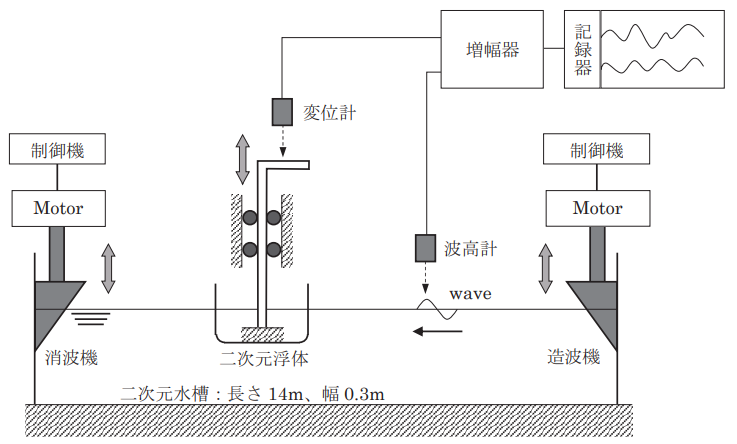
\includegraphics[width=0.8\linewidth]{summer/ship-experiment/2d-pool/pictures/gaiyo.png}
    \caption{二次元水槽及び波浪中動揺試験の計測の概要図}
    \label{fig:gaiyo}
\end{figure}

\section{試験設備, 計測機器, 試験条件}

\begin{itemize}
    \item 水槽
    \begin{itemize}
        \item 長さ14m
        \item 幅0.3m
        \item 水深0.45m
    \end{itemize}
    \item 模型船
    \begin{itemize}
        \item ルイスフォーム断面浮体
        \item 長さ$L=0.3m$
        \item 幅$B=0.2m$
        \item 喫水$0.1m$
        \item 水線下断面積$S=0.018m^2$
        \item 排水量$5.4kg$
    \end{itemize}
    \item 重力加速度$g=9.81\ m/s^2$
    \item キャリブレーション定数
        \begin{itemize}
            \item 波高計$\alpha=0.23$
            \item 変位計$\alpha=0.37$
        \end{itemize}
\end{itemize}

長手方向の両端にくさび型の造波機があり、任意の波を造波,消波できる。波高は動かす範囲、周波数は動かす速さで変えることができる。


波高の測定は図\ref{fig:laser}に示す、模型と造波機の間に設置したレーザー測距により行う。
レーザー測距により得た電圧データをアンプを通してPCに送っている。
今回、レーザー測距のキャリブレーションは時間の都合で予め行って頂いた。

\begin{figure}[H]
    \centering
    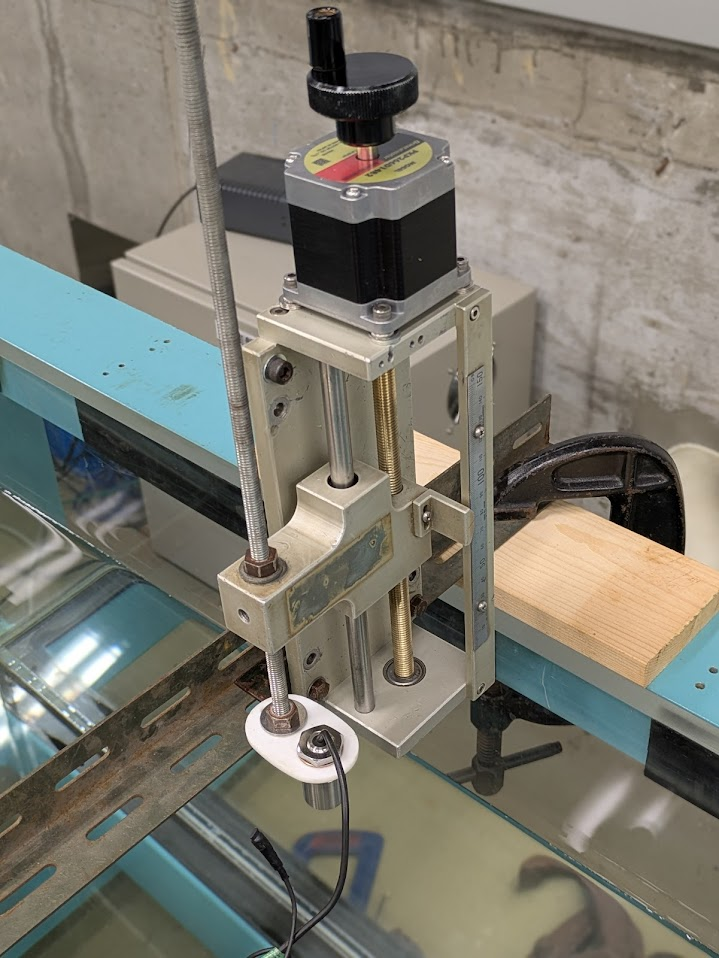
\includegraphics[width=0.5\linewidth]{summer/ship-experiment/2d-pool/pictures/laser.png}
    \caption{レーザー測距}
    \label{fig:laser}
\end{figure}

模型船は図\ref{fig:kotei}に示すように水槽の長手方向と鉛直方向は自由に動くようにスライドレールを2軸用いて固定した。
水槽長手方向には漂流していかないようにばねを張った。
\begin{figure}[H]
    \centering
    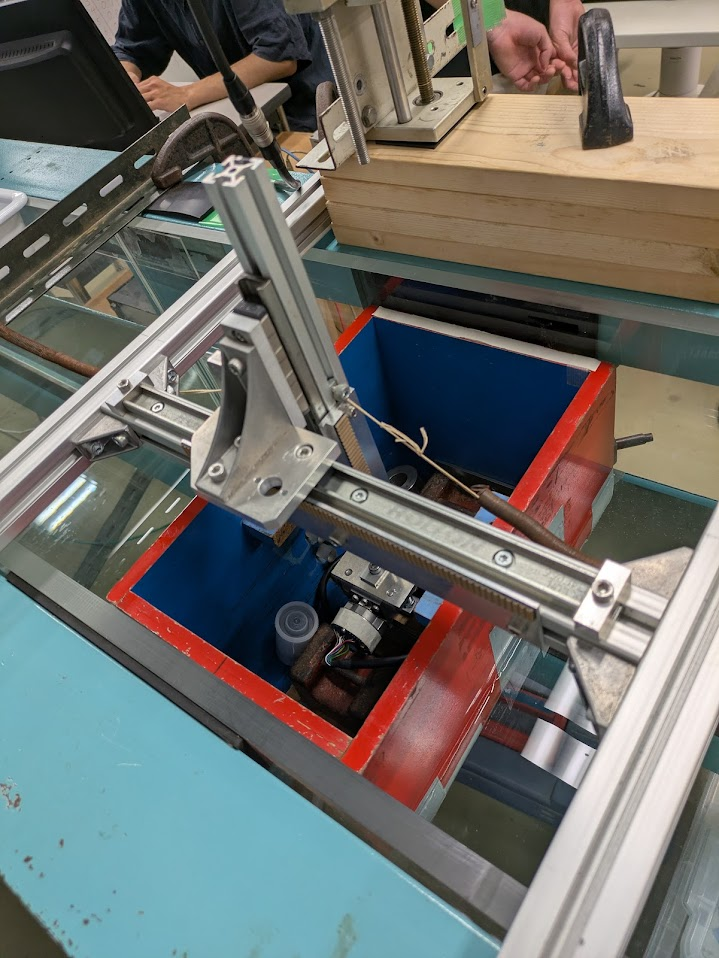
\includegraphics[width=0.5\linewidth]{summer/ship-experiment/2d-pool/pictures/kotei.png}
    \caption{模型船の固定方法}
    \label{fig:kotei}
\end{figure}

船体の上下動は模型に設置された図\ref{fig:encoder}のエンコーダーにより計測した。アブソリュート型かインクリメント型かは不明。磁気式ではないだろう。
鉛直軸側に設置されたMX型タイミングベルトをフレキラックとして用いてラック&ピニオンでエンコーダーが接続されている。

\begin{figure}[H]
    \centering
    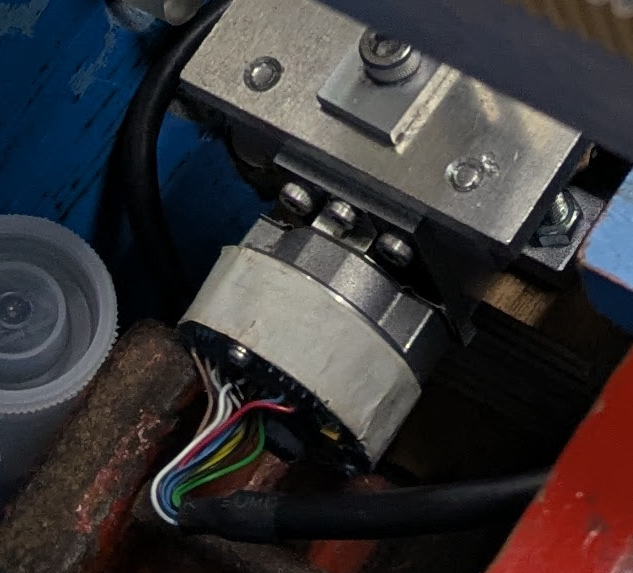
\includegraphics[width=0.5\linewidth]{summer/ship-experiment/2d-pool/pictures/encoder.png}
    \caption{上下動計測用のエンコーダー}
    \label{fig:encoder}
\end{figure}


\section{計測結果}
計測結果のグラフを以下に添付する

\begin{figure}[H]
    \centering
    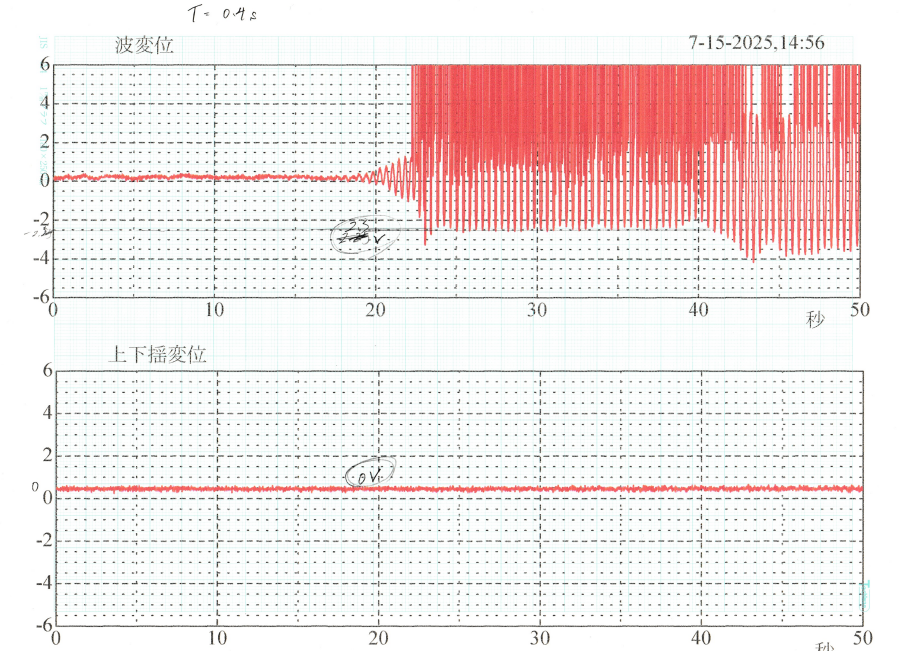
\includegraphics[width=0.9\linewidth]{summer/ship-experiment/2d-pool/pictures/t0.4.png}
    \caption{T=0.4}
    \label{fig:t0.4}
\end{figure}
\begin{figure}[H]
    \centering
    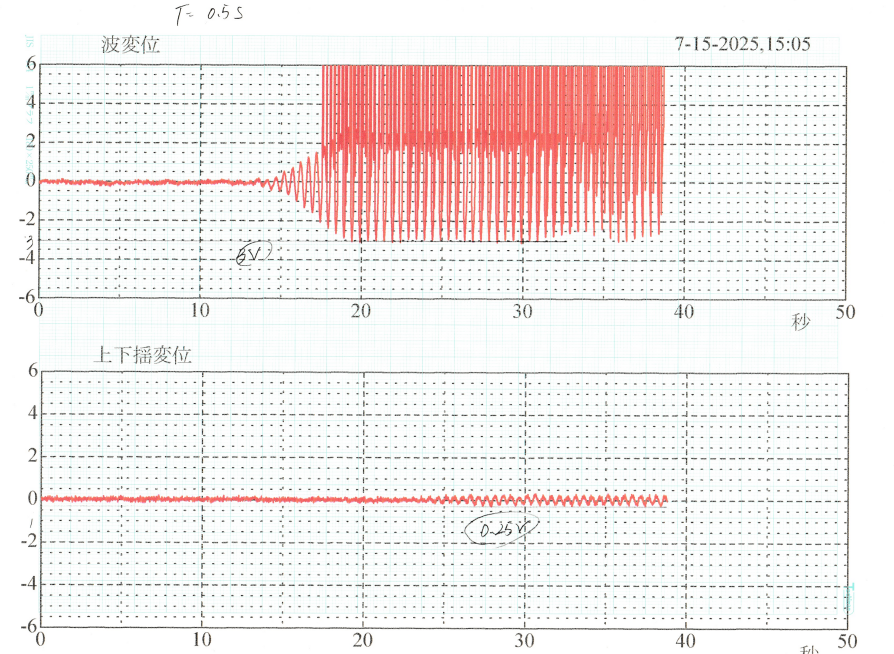
\includegraphics[width=0.9\linewidth]{summer/ship-experiment/2d-pool/pictures/t0.5.png}
    \caption{T=0.5}
    \label{fig:t0.5}
\end{figure}
\begin{figure}[H]
    \centering
    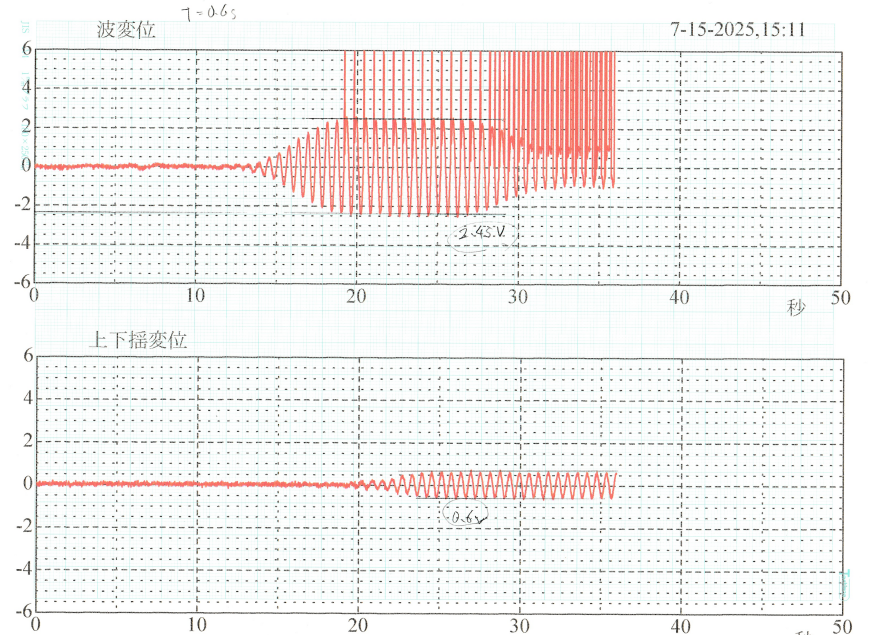
\includegraphics[width=0.9\linewidth]{summer/ship-experiment/2d-pool/pictures/t0.6.png}
    \caption{T=0.6}
    \label{fig:t0.6}
\end{figure}
\begin{figure}[H]
    \centering
    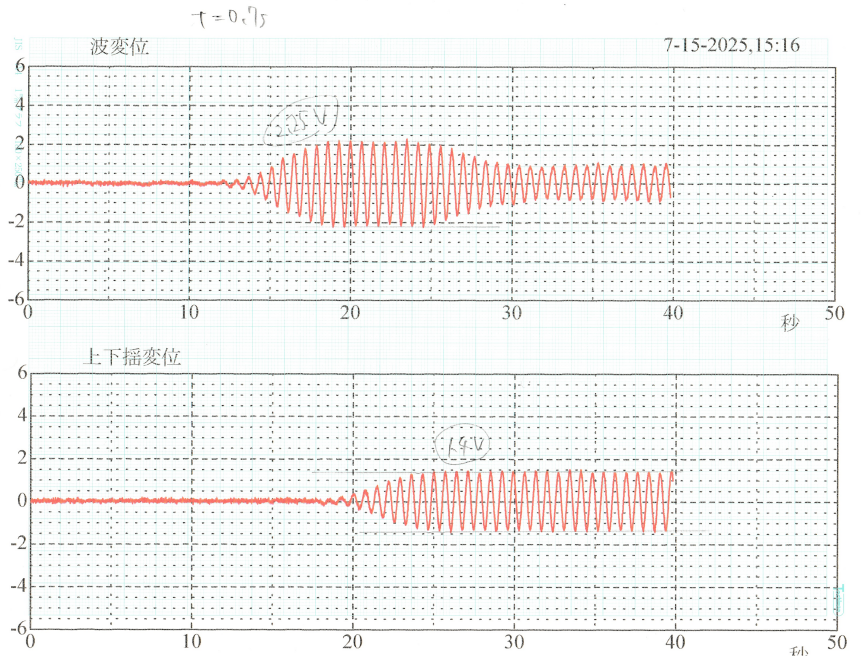
\includegraphics[width=0.9\linewidth]{summer/ship-experiment/2d-pool/pictures/t0.7.png}
    \caption{T=0.7}
    \label{fig:t0.7}
\end{figure}
\begin{figure}[H]
    \centering
    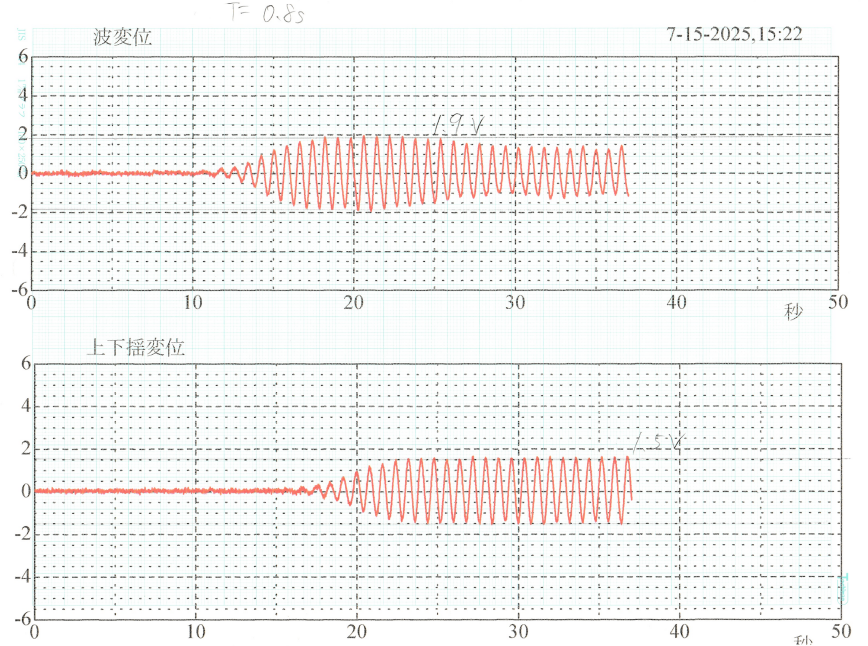
\includegraphics[width=0.9\linewidth]{summer/ship-experiment/2d-pool/pictures/t0.8.png}
    \caption{T=0.8}
    \label{fig:t0.8}
\end{figure}
\begin{figure}[H]
    \centering
    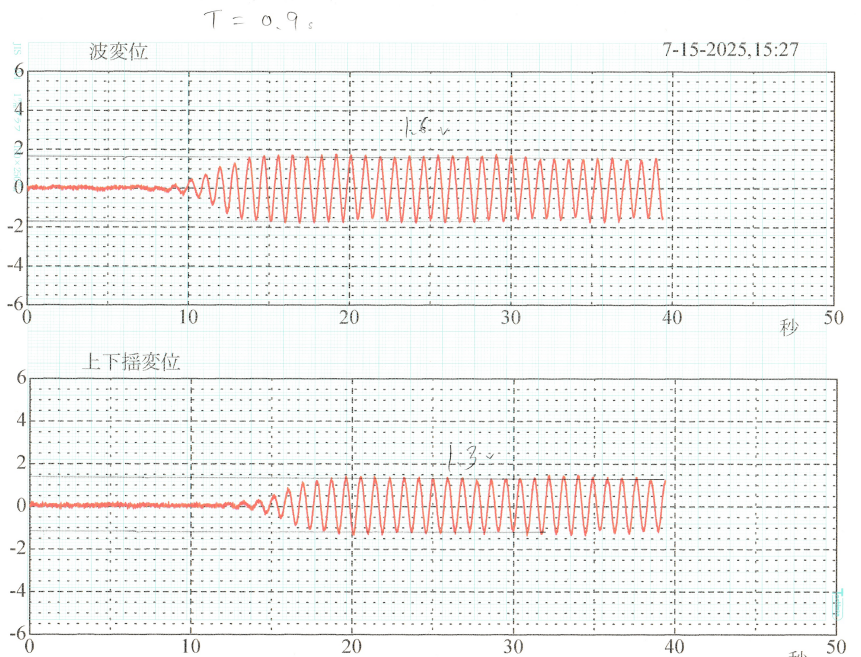
\includegraphics[width=0.9\linewidth]{summer/ship-experiment/2d-pool/pictures/t0.9.png}
    \caption{T=0.9}
    \label{fig:t0.9}
\end{figure}
\begin{figure}[H]
    \centering
    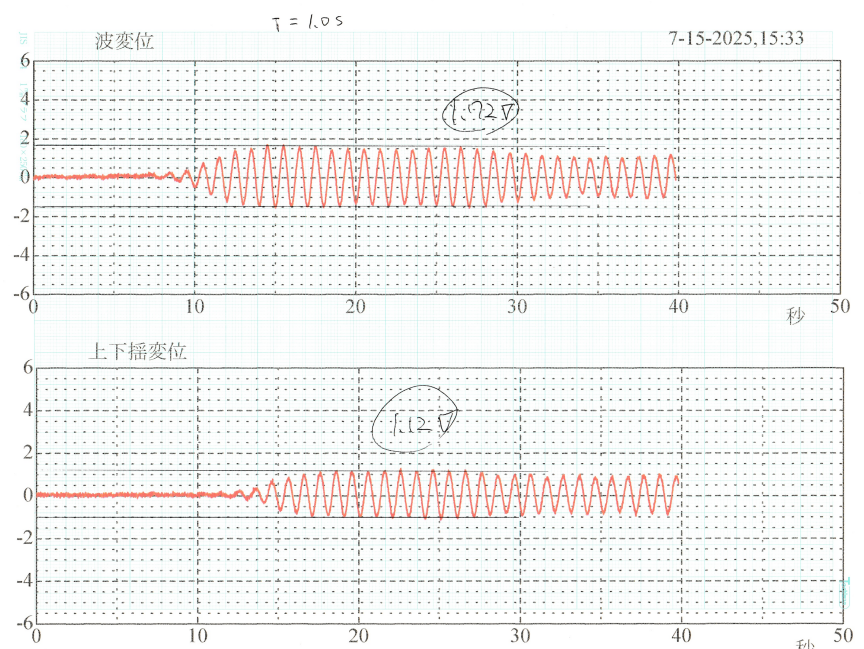
\includegraphics[width=0.9\linewidth]{summer/ship-experiment/2d-pool/pictures/t1.0.png}
    \caption{T=1.0}
    \label{fig:t1.0}
\end{figure}
\begin{figure}[H]
    \centering
    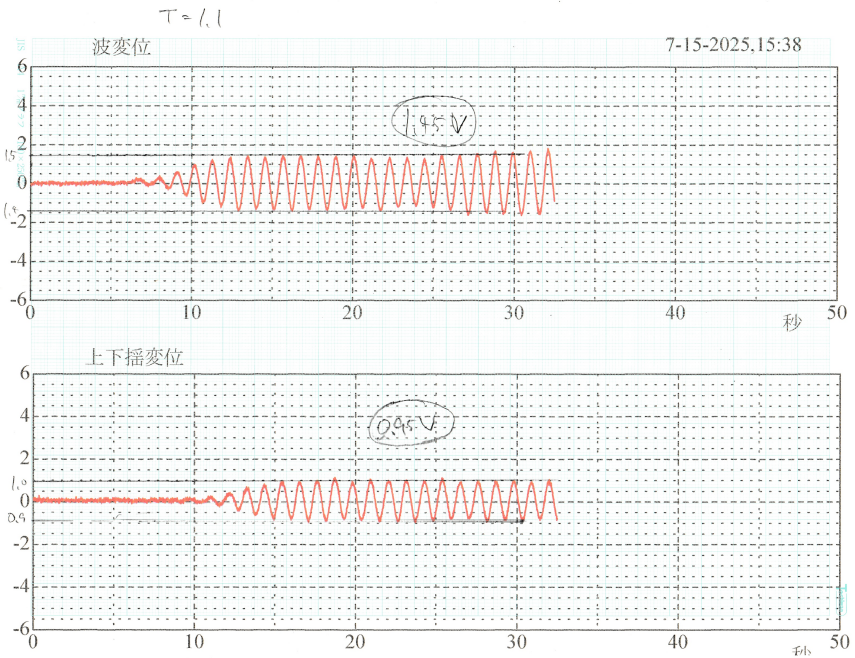
\includegraphics[width=0.9\linewidth]{summer/ship-experiment/2d-pool/pictures/t1.1.png}
    \caption{T=1.1}
    \label{fig:t1.1}
\end{figure}
\begin{figure}[H]
    \centering
    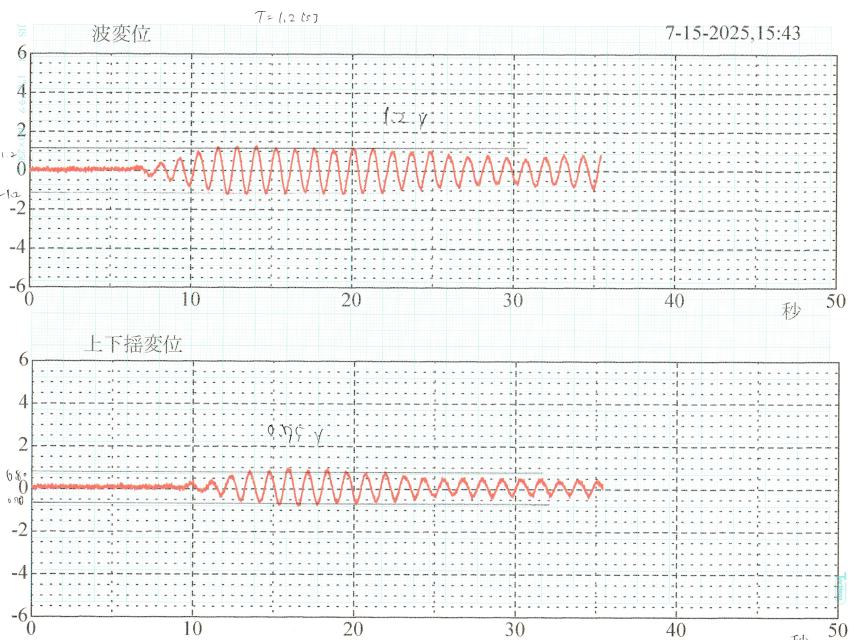
\includegraphics[width=0.9\linewidth]{summer/ship-experiment/2d-pool/pictures/t1.2.png}
    \caption{T=1.2}
    \label{fig:t1.2}
\end{figure}
\begin{figure}[H]
    \centering
    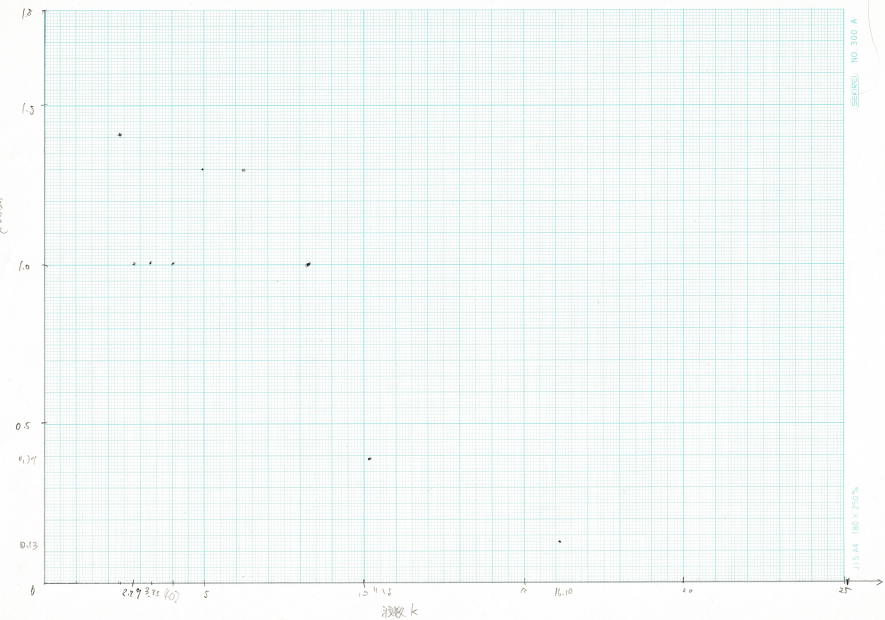
\includegraphics[width=0.9\linewidth]{summer/ship-experiment/2d-pool/pictures/graph01.png}
    \caption{振幅比-波数グラフ(実測)}
    \label{fig:graph01}
\end{figure}


\chapter{結果の比較と考察}
\section{理論値との比較}
与えられた流体力データから振幅比を算出すると以下のような分布になった。
計算の詳細は計算書や2章を参照されたい。

\begin{figure}[H]
    \centering
    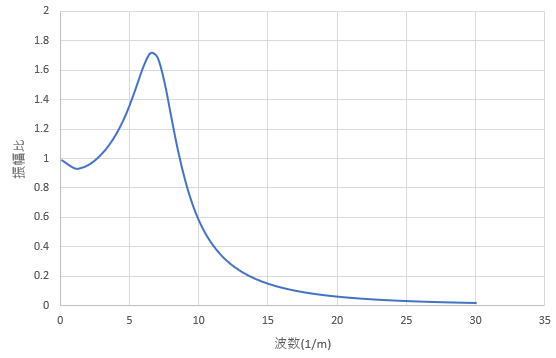
\includegraphics[width=0.9\linewidth]{summer/ship-experiment/2d-pool/pictures/shinpukuhi.png}
    \caption{振幅比-波数 グラフ(理論値)}
    \label{fig:shinpukuhi}
\end{figure}

図\ref{fig:graph01}と見比べてみると、波数の大きいグラフ右側部分では概ね一致していることがわかる。

一方で波数0~5程度の、最大点の左側では、実測の方のグラフは不規則な挙動を示している。\\不規則に見える要素は2点ある
\begin{itemize}
    \item 周期1.0~1.2の3点がほとんど横並びである点
    \begin{itemize}
        \item 理論値の方も変化率は小さいので納得できる部分はあるが、最大点のすぐ隣でこの結果となっているので不規則に感じられる。
    \end{itemize}
    \item 周期1.3の点で以上に振幅比が大きくなっている点
    \begin{itemize}
        \item 外れ値のように見える。もしくは最大点が実際には2点存在しているのか、再検証が必要である。
    \end{itemize}
\end{itemize}
波数の小さい範囲では理論値と実際での乖離が見られたので、総じて最大点までの範囲での再検証が必要である。

\section{考えられる不具合}
\subsection{グラフから読み取った値の正確性}
今回結果として得られたグラフの振幅はずれが大きく、また、振幅の読み取り方もその場で概ね分布の多いとみられる部分に線を引き読み取るという方法を採用していたので、この作業で大きなずれが起きたことが考えられる。
この改善のためには以下の2点が挙げられる
\begin{itemize}
    \item 結果をアナログなグラフで出すのではなく、その点群データで得ることで、正確な振幅を算出する。
    \item 波の群速度から水波が水槽を往復してくるまでの時間を計算し、必ずそこまでの秒数で計測を終える事で重ね合わせを回避する。
\end{itemize}
\subsection{測器の固定不良}
模型船の基軸部分はアルミフレームにより頑強に固定されていたが、波高を計測するレーザー測距は図\ref{fig:angle}のようにアングル材で固定されており、容易に傾斜し得る状況にあった。これにより多少測器が水面に対して傾斜していた可能性が考えられる。
\begin{figure}[H]
    \centering
    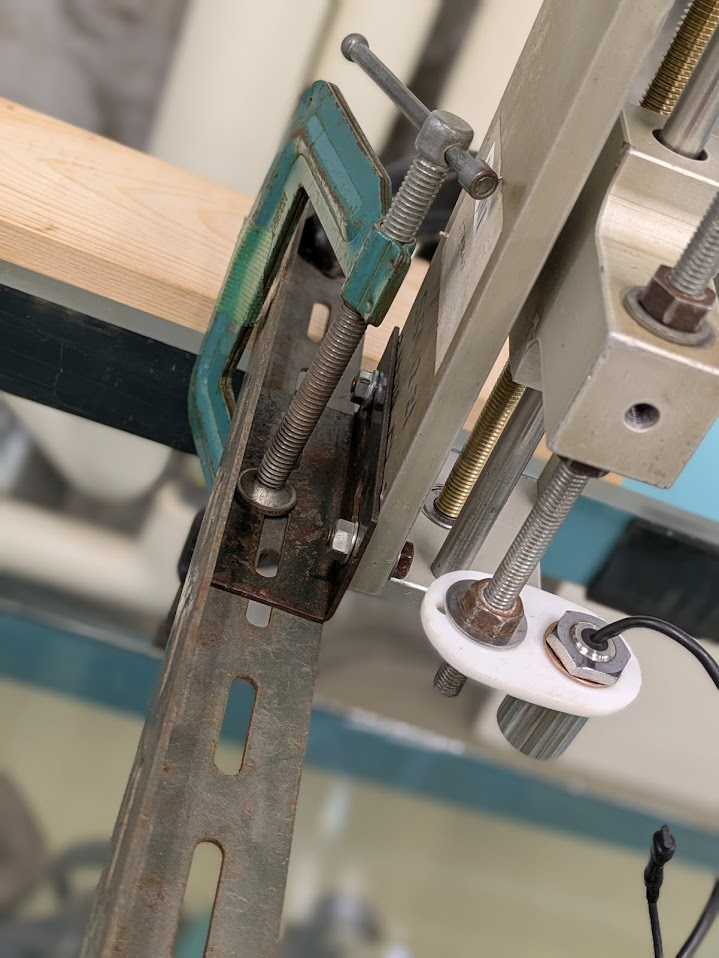
\includegraphics[width=0.5\linewidth]{summer/ship-experiment/2d-pool/pictures/angle.png}
    \caption{レーザー測距の固定}
    \label{fig:angle}
\end{figure}

また、模型船についても、スライドレールのがたつきが気になった。
水槽との間の固定は頑強であったのに対し、可動部分はローラー式のスライドパックが採用されており、揺れやすい構造になっていた。模型船の排水量が大きい事も考慮して、揺れにくく強度の強いリニアガイドを用いて固定すればより良い結果が得られると考えられる。

\subsection{ラック&ピニオンのバックラッシ}
ラック&ピニオン機構を使う際はどうしても多少の遊びができてしまい、その分応答が遅れることが考えられる。今回用いられたタイミングベルトのモジュールは1mm程度であり、実験結果に大きく影響する要因ではないが、多少のずれが生まれていたのは間違いないだろう。
これの改善策として、トコロイド曲線を用いたギヤを使うことや、シリンダ式の測距機を使う事が挙げられる。

\chapter{感想・考察}

本実験は、参加者全員が全ての工程を体験する形式であり、一連の流れや各段階の役割を明確に把握できた。これにより、誤差の発生源の特定や装置の操作方法に対する理解が深まったことは、大きな収穫であった。

これまでの実験では特定の作業に携わることが多かったため、今回、造波から計測まで全ての工程を経験できたことは、非常に新鮮で興味深かった。特に、自らの手で造波機を操作し、意図した波が生まれる様子を目の当たりにした際には、\textbf{自らの操作が物理現象として現れるという科学実験の醍醐味を実感した。}

さらに、実験データの整理と並行して関連理論を再学習したことで、船体運動に関する数式と実際の現象との結びつきを強く意識できた。このように\textbf{理論と実践が結びつく経験は、学習内容への理解を質的に向上させるだけでなく、今後の専門分野への探究心を一層高める有意義なものとなった。}
\chapter{参考文献}
船舶海洋工学実験 講義資料
\end{document}